% !TeX root = ../main.tex

\chapter{图形栈结构分析与需求分析}
本课题研究是的安卓图形栈在龙芯软硬件环境下的实现,并最终编译构建可运行在龙芯环境下的安卓系统镜像。安卓的图形系统作为安卓最复杂的模块之一,
在开始移植的工作之前,首先需要对其整体结构做一个分析,明确需要的工作。为了兼容硬件供应商的不同的底层硬件实现,安卓framework层定义了大量的抽象接口
规定了每个安卓版本的所需实现的功能,而具体的功能实现则需要各家硬件供应商去实现。本章首先阐述安卓图形栈的整体结构,分析安卓图形模块调用底层驱动库的过程,
然后对图形系统中涉及龙芯硬件的部分进行需求分析,最后具体介绍各部分的设计。
\section{整体设计}
\subsection{安卓图形系统的整体构成}
\begin{figure}[h]
  \centering
  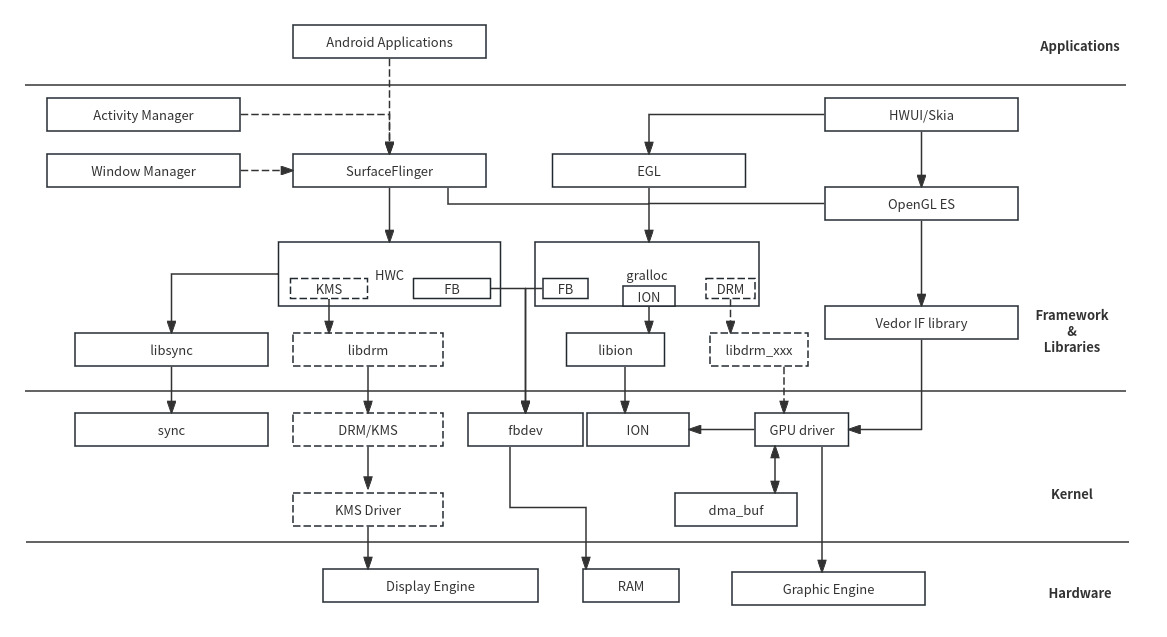
\includegraphics[width=0.8\textwidth]{安卓图形栈结构图.jpg}
  \caption{安卓图形栈结构图}
  \label{fig:安卓图形栈结构图}
\end{figure}
如图\ref{fig:安卓图形栈结构图}所示,安卓的内核部分仍然是依赖linux内核的KMS和DRM。DRM是目前linux主流的图形显示框架,而KMS是linux中管理显示设备的模式和刷新
的部分。安卓的framework层以及库函数依赖的图形接口由libdrm进行封装,用以屏蔽底层硬件实现的具体细节。这其中有两个重要的模块,一个是
HWC(硬件混合渲染器),是进行窗口合成和显示HAL层模块,其实现是特定于设备的,通常是由显示设备制造商 (OEM)完成。其用于合成从Surfaceflinger接收
的图层,从而减少OpenGL ES (GLES) 和 GPU 执行的合成量。而另一个模块是gralloc。它是Android中负责申请和释放GraphicBuffer的HAL层模块,
由硬件驱动提供实现,为BufferQueue机制提供了基础。gralloc的主要组件包括Allocator,Mapper。Allocator 负责内存的分配和释放,
主要功能包括:根据请求的大小和格式分配内存缓冲区,负责跟踪已分配和空闲的内存块以及支持在多个进程之间共享缓冲区,使得不同的应用程序或组件能够访问同一块内存。
Mapper负责将已分配的缓冲区映射到进程的虚拟地址空间。本课题需要实现支持龙芯硬件平台的gralloc和HWC模块的库以支持上层接口调用。

\subsection{surfaceflinger初始化过程分析}
\begin{figure}[h]
  \centering
  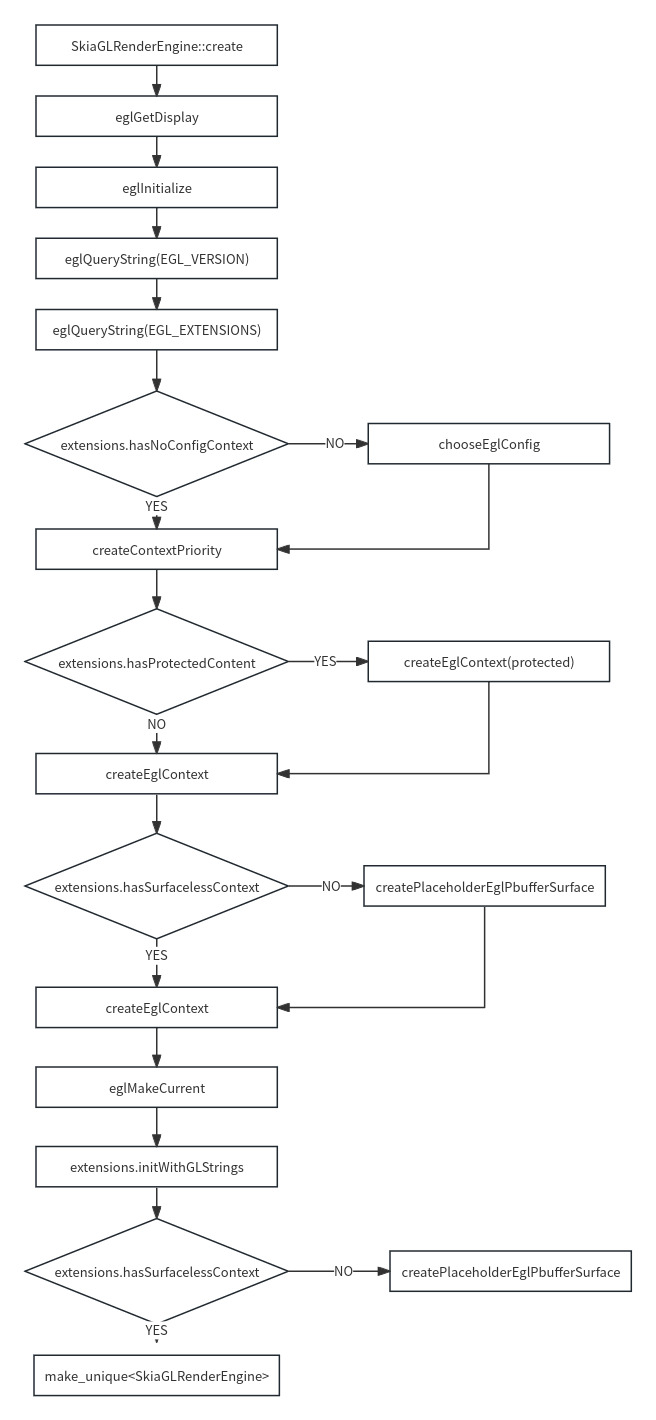
\includegraphics[width=0.35\textwidth]{skia_create过程.jpg}
  \caption{skiaRenderEngine创建时初始化EGL流程图}
\end{figure}

安卓2D渲染引擎默认使用的是skia,所以surfaceflinger初始化过程首先是skia引擎的初始化,在SkiaGLRenderEngine::create时,
会依次执行eglGetDisplay获取EGL显示句柄,此句柄代表了要渲染的物理设备;eglInitialize初始化EGL环境,并获得EGL的主次版本号;
eglQueryString查询与当前显示连接相关的字符串信息,包括EGL版本信息、供应商版本信息以及支持的客户端API等,安卓还会使用EGL\_EXTENSIONS
获取有关安卓特性的拓展并初始化;使用createEglContext在EGL中创建 OpenGL ES 上下文;然后使用eglMakeCurrent将指定的渲染上下文和表面设置为当前的函数。

下面以eglInitialize为例,说明surfaceflinger是如何通过安卓的framework层的接口调用龙芯用户态驱动程序的。

\begin{figure}[h]
  \centering
  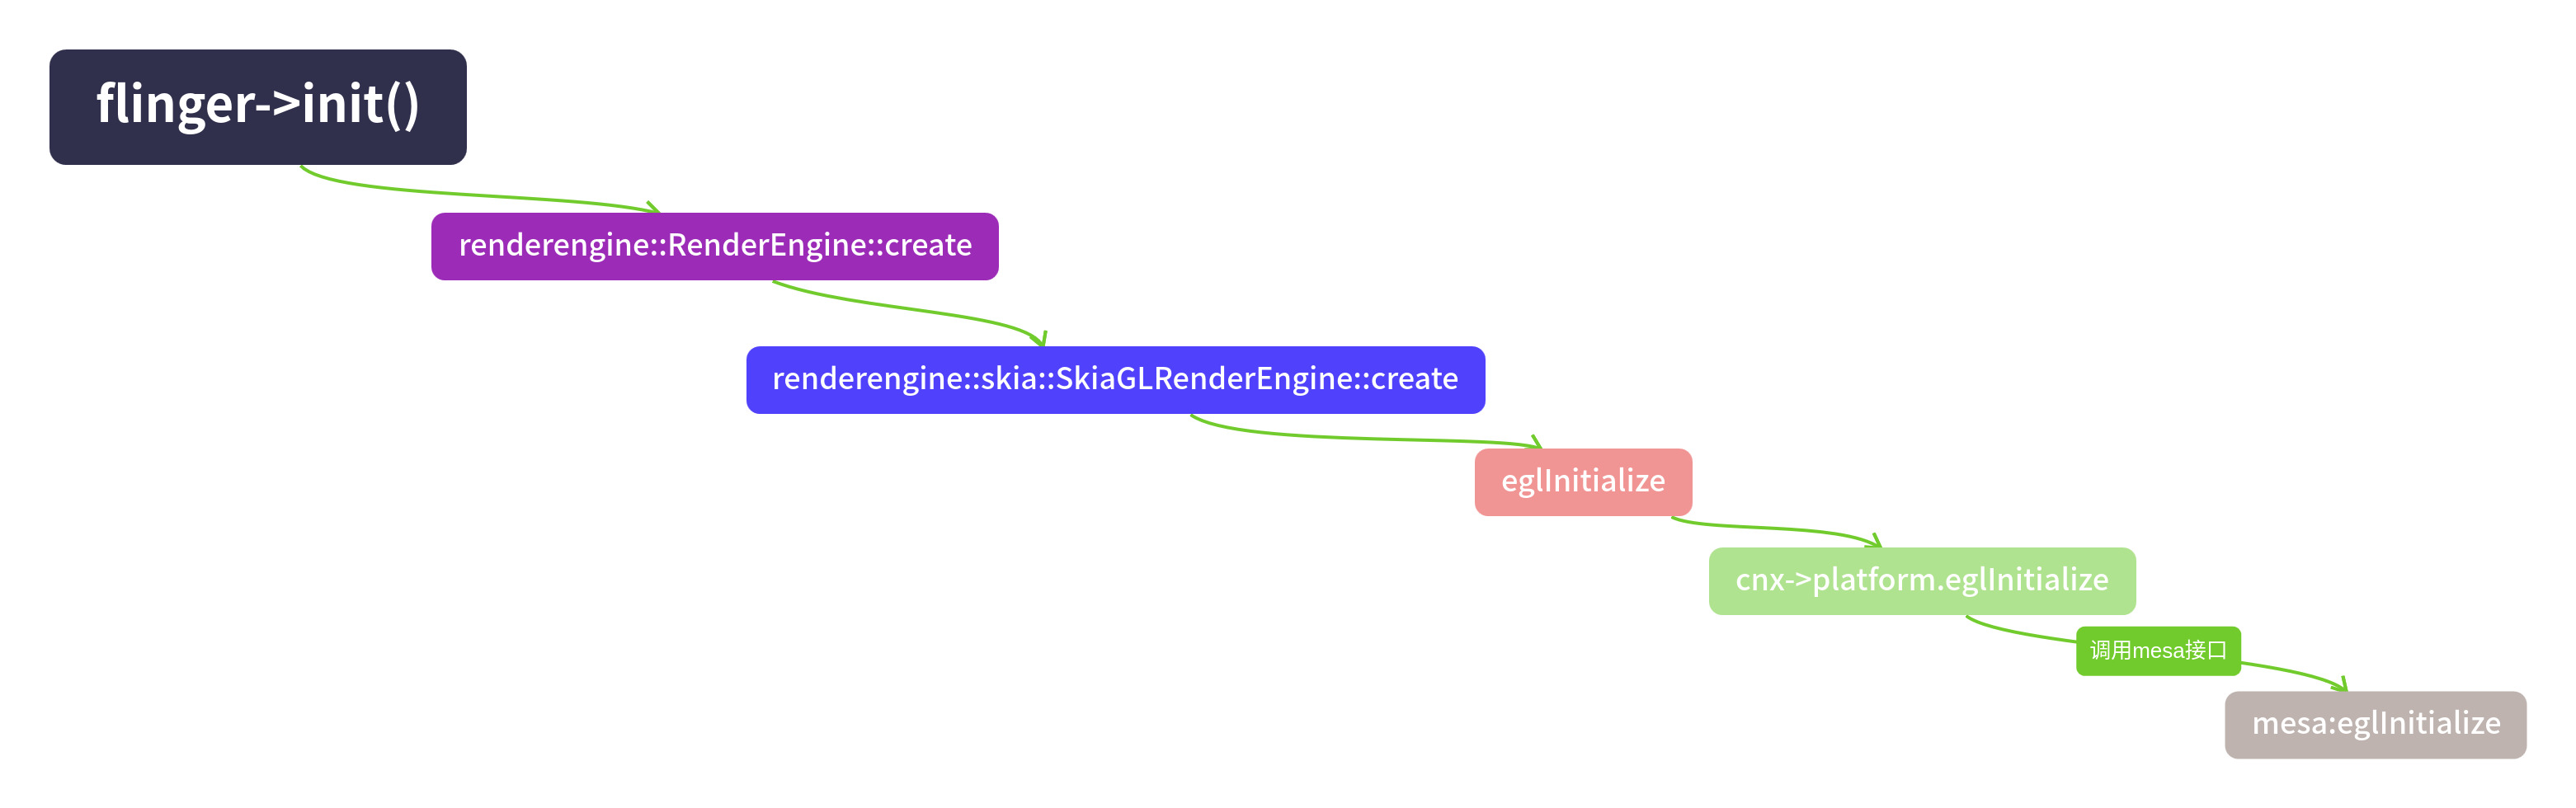
\includegraphics[width=0.8\textwidth]{flinger_egl初始化示意图.jpg}
  \caption{flinger驱动调用函数栈}
\end{figure}

首先是surfaceflinger初始化,调用flinger->init函数,根据PROPERTY\_DEBUG\_RENDERENGINE\_BACKEND宏判断使用渲染引擎的类型,可以是GLESRenderEngine
或SkiaGLRenderEngine,安卓中一般默认的都是SkiaGLRenderEngine,然后是引擎的create。调用eglInitialize,会使用LayerLoader::LoadLayers
中dlopen加载的libGLES\_mesa.so去初始化修饰的egl\_connection\_t结构体,调用gEGLImpl的接口,从而实现对龙芯用户态显卡驱动的调用。

\section{移植需求分析}
安卓使用的图形协议是深度定制的,而x11,wayland协议是运行在传统linux内核下的协议,因此龙芯现有的图形栈解决方案在安卓上并不完全适用。
由图3.1可知,图形的内核层使用的仍然是linux内核的drm/kms框架,应用层使用的是libdrm,由libdrm向上对HAL层的gralloc和HWC提供接口,实现图形
graphic buffer的申请和释放,以及HWC硬件混合渲染器的窗口合成。GPU驱动的加载在Surfaceflinger的初始化过程中skia
(2D渲染引擎)创建时进行加载,根据设置的驱动加载方式(本文使用的是dri2)在eglInitialize时通过eglApi的接口调用mesa中的eglInitialize
函数dri2\_initialize,从而实现mesa驱动的加载和初始化。

\subsection{mesa适配方案}
\textbf{需求背景}:mesa使用的版本为18.3.6,而由于现有的安卓版本为12.0.0,安卓API版本为31对应的mesa版本为20.3.4,因此需要对现有的mesa的dri接口进行升级。并且由于安卓新的
编译方式Soong的加入,mesa目前最新的版本已经废弃了传统的mk编译方式,转而采用伪编译的方式。为考虑后续版本的兼容性,因此在现有的mesa18.3.6上采用伪编译的方法,
使用mesa原本的ninja编译方式,将生成的动态库文件添加到安卓目标生成目录中。此后,mesa库将被编译为libgallium\_dri.so以及libglapi.so。其中libgallium\_dri.so
用于支持DRI使得应用程序可以直接与GPU进行通信,绕过X服务器从而实现更高效的渲染;同时实现多个图形API,包括OpenGL,利用Gallium3D的架构来支持gsgpu的后端。而libglapi.so
则负责管理OpenGL API调用的分发,将调用路由到适当的实现,通常是后端的图形驱动程序并且处理OpenGL上下文的创建、管理和切换,确保正确的状态和资源在不同的渲染上下文中得到维护。
由此背景,可以分析得到以下数个方面的需求。

1. 编译与构建适配

尽量使用最新的伪编译框架去生成动态库文件,并为上层安卓龙芯产品产品配置文件留下对应的接口。确保 libgallium\_dri.so 和 libglapi.so 动态库
在龙芯架构下能够正确生成,确保动态库的兼容性及性能。

2. 图形 API 支持

打通GPGPU后端支持Gallium3D的通路,确保 OpenGL 的核心功能集成到龙芯平台,确保API 的正确性。

3. 性能优化

针对龙芯架构的特点,优化 Mesa 的编译选项以提升性能。
针对 Gallium3D 后端渲染效率的优化,包括批处理、资源管理和 API 调用路径。

\subsection{HWC}
%每个厂商hwc实现可能不同如nxp,rockchip,drm-hwc,ranchu,也有很多厂商实现是闭源的如nxp,而谷歌的drm-hwc,ranchu是开源的
HWC 是 Android 图形架构中的一个重要组件,作为硬件抽象层(HAL)的一部分,负责与底层显卡驱动和显示硬件进行交互。其与Surfaceflinger
紧密协作,Surfaceflinger负责接收应用程序的绘制请求,并将其发送到HWC进行合成;同时使用libdrm向上提供的API接口来管理显示硬件。

\subsection{gralloc}
gralloc模块接口定义于frameworks/native/libs/ui下,可以分为两个部分Allocator和Mapper。
主要实现的功能是为了创建、管理和操作缓冲区对象,其中需要完成一些与硬件特性相关的接口函数,如:

\textbf{init\&close}:驱动程序的初始化和关闭
\textbf{bo create}:创建缓冲区对象(BO)的函数,实现内存分配和初始化
\textbf{bo destroy}:销毁缓冲区对象的函数,负责释放已分配的内存
\textbf{bo import}:导入缓冲区对象的函数,允许将外部缓冲区导入到 GBM 管理的缓冲区中。
\textbf{bo map}:映射缓冲区对象的函数,使得 CPU 可以访问 GPU 分配的内存。
\textbf{bo unmap}:解除映射缓冲区对象的函数,释放 CPU 对缓冲区的访问。
依据硬件的设计可以选择在初始化时是否使用tiled等模式进行访存优化,提供更灵活的驱动交互方式。

\section{准备工作}

\subsection{硬件适配分析}
由于龙芯显卡 LG110 的存储管理单元(Memory Management Unit, MMU)采用页式管理来处理 GPU 所使用的内存,
所有内部功能模块均使用虚拟地址。在连接到内部网络之前,这些地址需要经过转换。当前,MMU 设计了三级页表结构,且页大小(page size)为 16KB。
然而,Android 12 尚未支持 16KB 的页大小。这意味着需要对以下几个方面进行修改:

\textbf{Bionic 库}:需要在 Bionic 中调整页面数据结构,以支持 16KB 的页大小。

\textbf{安卓通用内核文件系统}:在内核的文件系统(如ext4、super和f2fs)中添加对 16KB 页大小的支持。

\textbf{AOSP部分系统服务}:在 AOSP 中的部分系统服务中也需添加相应的支持。

具体实现方法是使用内联函数 page\_size() 来获取内核中的页大小,从而实现对多种页面大小的兼容。这种改动将确保龙芯显卡的 MMU 
能够高效地与 Android 系统和应用程序进行集成,提供更好的性能和兼容性。

\subsection{内核编译\&bionic\&部分系统服务修改说明}

\textbf{内核编译}:本课题所使用的内核是安卓通用内核5.10,因此在编译时需要添加安卓特性相关的驱动支持如ASHMEM、BINDERFS、BINDERIPC等,
虚拟内存管理使用三级页表,页表大小为16Kb。将f2fs模块的相关的宏定义做适应性调整。
详见表\ref{tab:f2fs模块修改说明}。以此为基础,对f2fs模块中所有依赖这几个宏的相关实现进行修改。
\begin{table}[h]
  \centering
  \caption{f2fs模块修改说明}
  \label{tab:f2fs模块修改说明}
  \begin{tabular}{lll}
    \toprule
    宏名   &   原有  &改动  \\
    \midrule
    F2FS\_MAX\_LOG\_SECTOR\_SIZE & 12 & PAGE\_SHIFT \\
    F2FS\_LOG\_SECTORS\_PER\_BLOCK & 3 & PAGE\_SHIFT - 9 \\
    F2FS\_BLKSIZE & 4096 & PAGE\_SIZE \\
    F2FS\_BLKSIZE\_BITS & 12 & PAGE\_SHIFT \\
    \bottomrule
  \end{tabular}
  \note{}
\end{table}

\textbf{bionic\&部分系统服务修改:}这两个部分的适配的动机与内核类似,具体实现可以在bionic\/libc\/platform\/bionic\/page.h中实现一个page\_size()的函数用以实现从内核
中动态获取页表大小,并以此为适配有使用PAGE\_SIZE为4k相关的服务,累积完成40项的修改。
\begin{figure}[h]
  \centering
  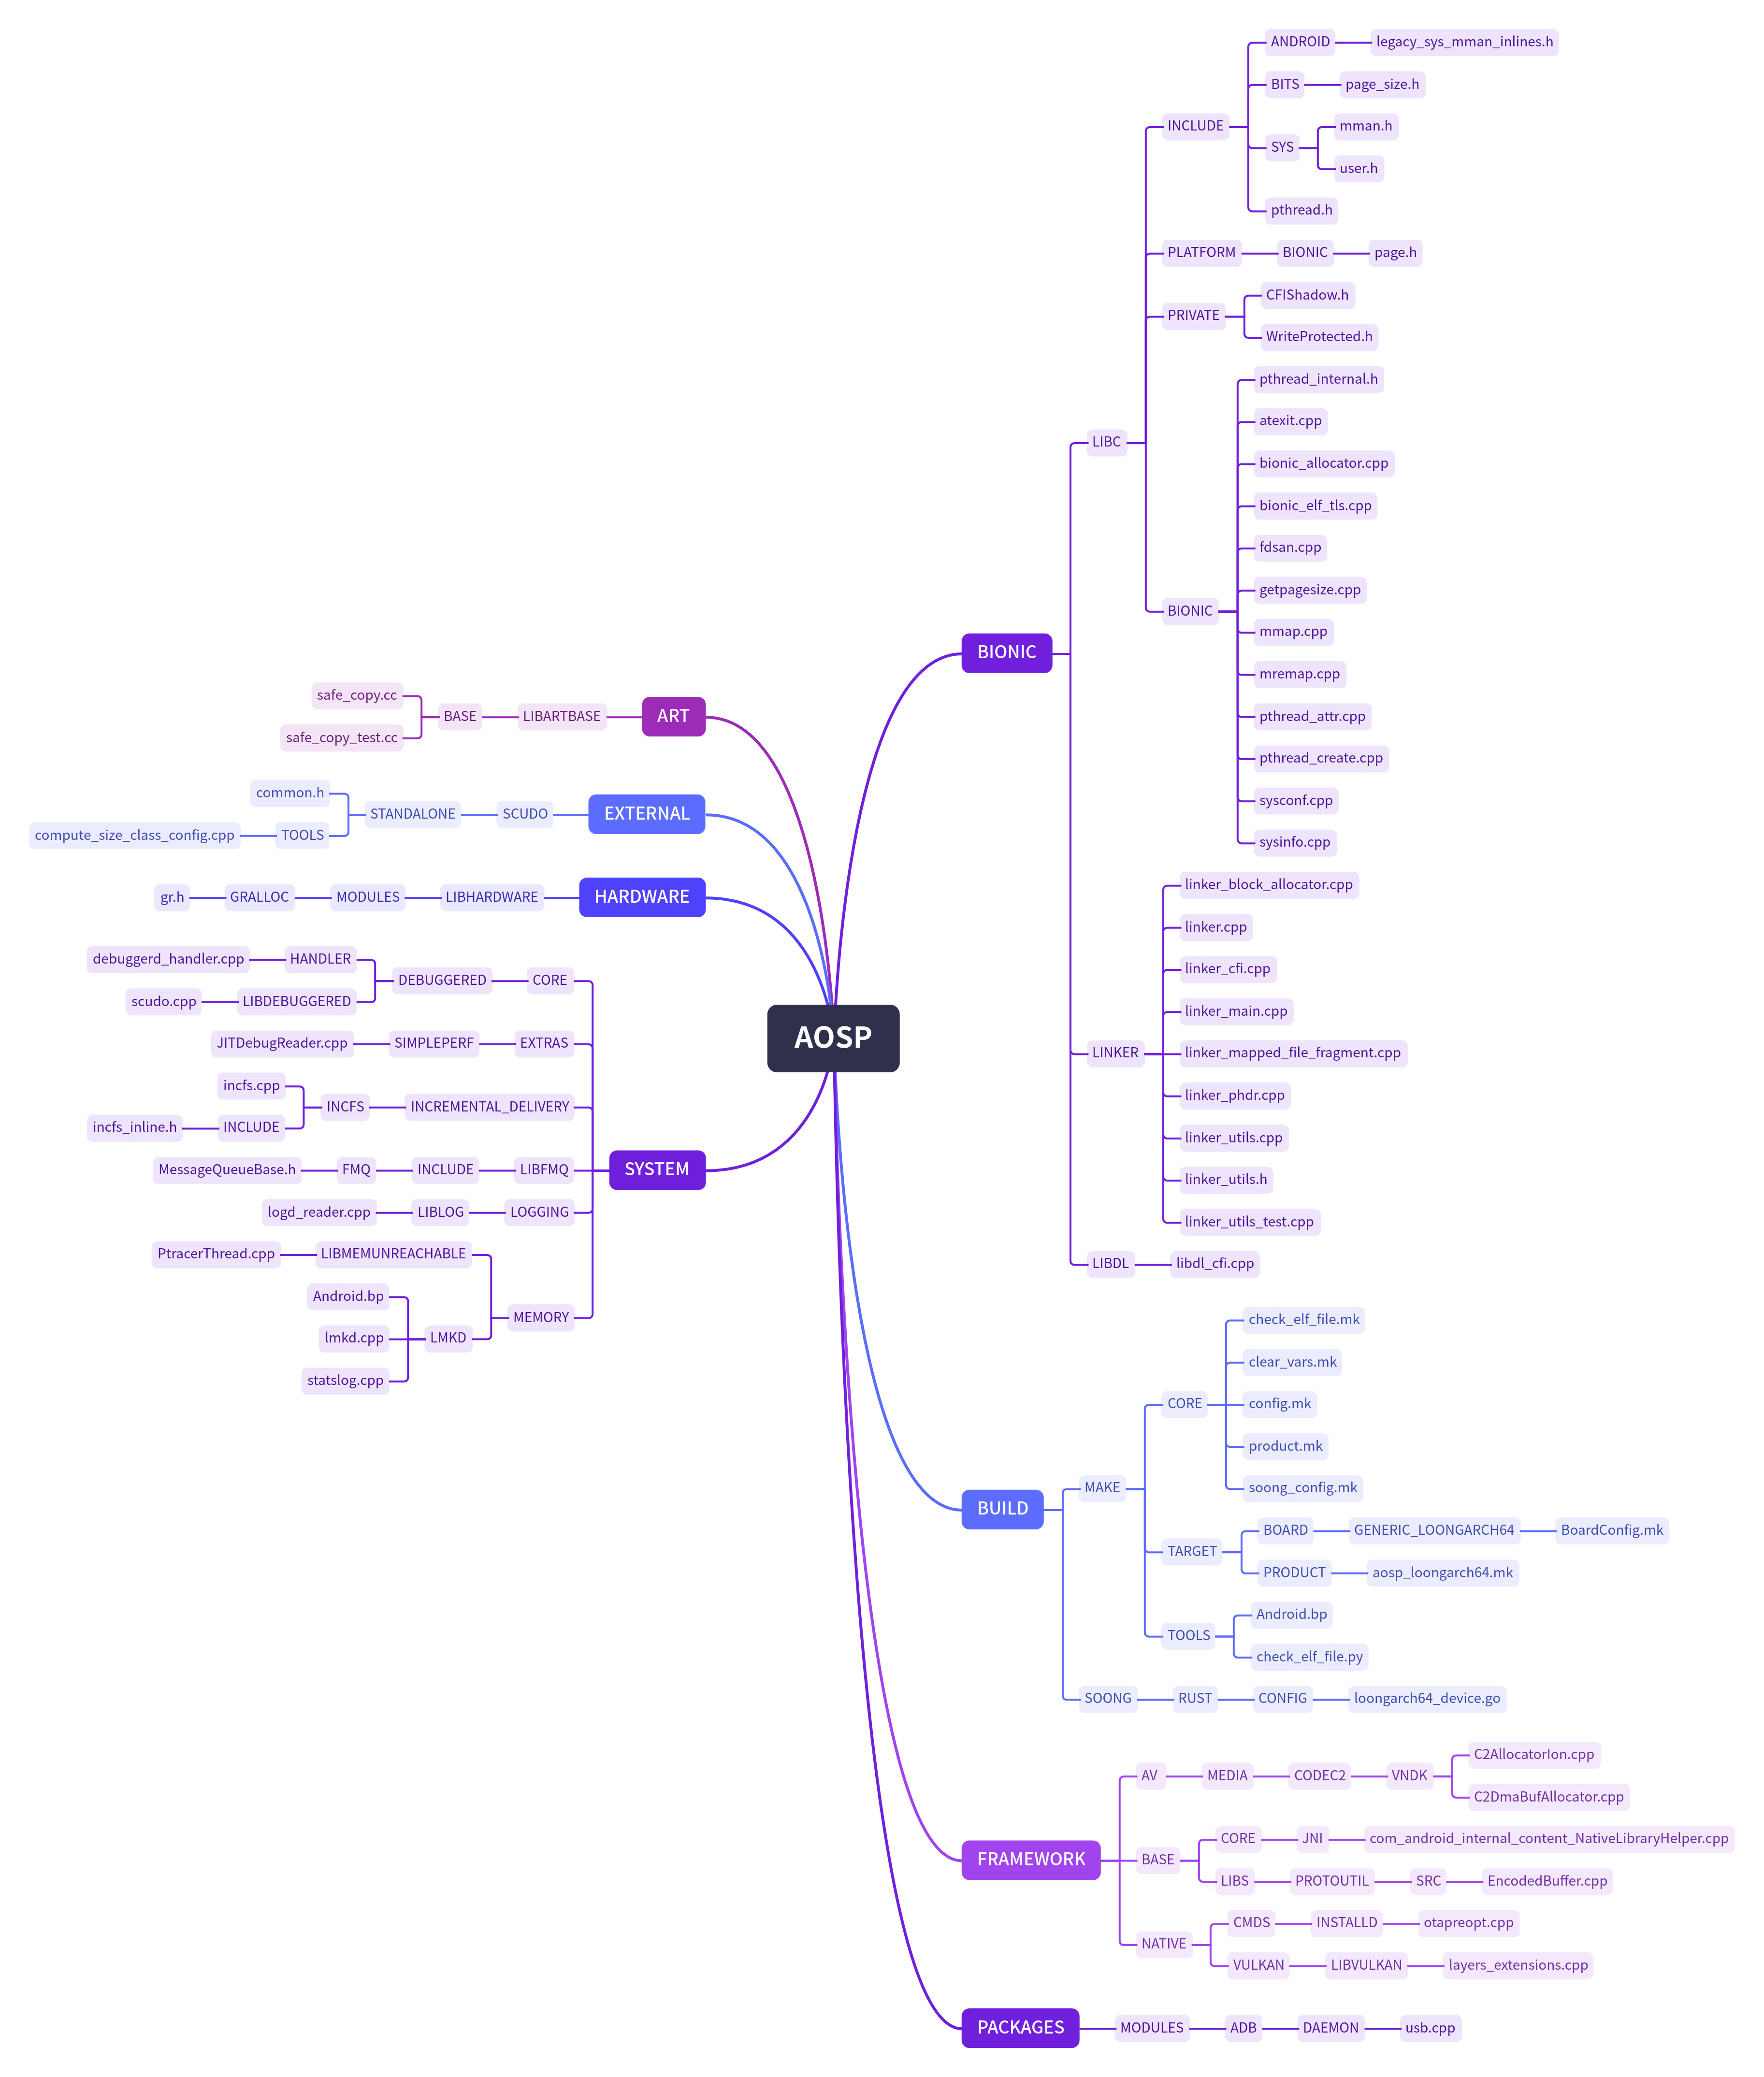
\includegraphics[width=0.8\textwidth]{androidS 16k适配改动图.jpg}
  \caption{androidS 16k适配改动图}
\end{figure}

\subsection{内核驱动}
现使用安卓内核版本为5.10,由于龙芯gsgpu内核驱动属于闭源状态,尚未整合到已有的内核源码,采用的方案为驱动模块独立开发的方式,在源码树之外编译.ko驱动文件,
并在进入安卓系统后使用insmod方式加载.ko驱动文件。另外由于内核gpu/drm模块的接口变化较多,因此在原有的4.19内核版本驱动的基础上进行多版本适配,
即可以动态识别内核驱动版本接口。具体的方案为通过调用drm模块的接口函数判断是否存在或者是否存在某个参数来判断内核版本,以此为基础适配相应的GPU资源描述
数据结构。

\textbf{内核版本变化说明}
从常用的4.19的内核到目前安卓内核版本5.10,内核驱动模块的接口变化主要集中在drm模块上。
\begin{table}[h]
  \centering
  \caption{内核4.19-5.10 drm接口变化}
  \begin{tabular}{lll}
    \toprule
    类型   &   名称  &变化时内核版本  \\
    \midrule
    变量 & DRIVER\_PRIME & 5.4 \\
    变量 & DRIVER\_IRQ\_SHARED & 5.1 \\
    函数 & drm\_sched\_stop & 5.1 \\
    函数 & drm\_fb\_helper\_fill\_info & 5.2 \\
    变量 & glob(ttm\_bo\_device\_init) & 5.0 \\
    函数 & ttm\_resource\_manager & 5.9 \\
    ... & ... & ... \\
    \bottomrule
  \end{tabular}
  \note{共计48项}
\end{table}

\section{详细设计}
\subsection{内存管理}
内核态驱动:

转换表映射模块:
TTM(Translation Table Maps)适用于GPU内存管理的一部分,提供了对显存(VRAM)、主存、共享内存等不同类型内存的管理功能。
它通过一个通用的 API 提供内存分配、缓冲区对象管理和内存交换等功能,使得 GPU 驱动能够灵活管理图形资源。
TTM 需要实现的功能有:缓冲区对象(BO)创建与销毁、 内存管理与分配、内存驱逐和交换、内存访问控制、I/O 内存管理和缓冲区对象的绑定与解绑。
\begin{figure}[h]
  \centering
  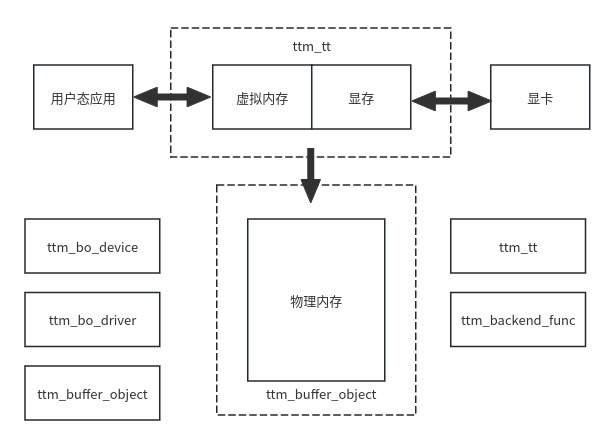
\includegraphics[width=0.8\textwidth]{DRM TTM结构.jpg}
  \caption{TTM主要对象}
\end{figure}



% 字段名	对应的函数	功能描述
% name	"gsgpu_common"	模块的名称,通常用于标识该模块或打印调试信息。
% early_init	gsgpu_common_early_init	早期初始化函数,模块初始化前需要做的一些准备工作。
% late_init	gsgpu_common_late_init	后期初始化函数,在其他初始化完成后执行的工作。
% sw_init	gsgpu_common_sw_init	软件部分的初始化函数,通常用于分配内存、初始化数据结构等。
% sw_fini	gsgpu_common_sw_fini	软件部分的清理函数,用于释放资源、销毁数据结构。
% hw_init	gsgpu_common_hw_init	硬件部分的初始化函数,负责配置硬件寄存器或启动硬件功能。
% hw_fini	gsgpu_common_hw_fini	硬件部分的清理函数,负责关闭硬件功能或恢复硬件状态。
% suspend	gsgpu_common_suspend	挂起函数,通常在系统进入睡眠模式(如 S3)时调用,用于保存硬件状态。
% resume	gsgpu_common_resume	恢复函数,通常在系统从睡眠模式恢复时调用,用于恢复硬件状态。
% is_idle	gsgpu_common_is_idle	判断模块是否处于空闲状态的函数,通常用于调试或节能管理。
% wait_for_idle	gsgpu_common_wait_for_idle	等待模块进入空闲状态的函数,通常用于保证操作完成后再进行后续操作。
% soft_reset	gsgpu_common_soft_reset	软复位函数,用于在某些情况下重置模块,而无需对整个系统进行硬复位。
% \subsection{gralloc}




% 1. Allocator
% Allocator 负责内存的分配和释放,主要功能包括:

% 内存分配:
% 分配一块合适大小的内存区域,通常用于图形缓冲区(如帧缓冲、纹理等)。
% 格式支持:
% 支持多种像素格式(如 RGBA、YUV 等),确保分配的内存符合所需的格式和对齐要求。
% 内存管理:
% 管理可用内存的状态,跟踪已分配和未分配的内存区域,确保内存的高效使用。
% 性能优化:
% 通过优化内存分配策略(如缓存机制、批量分配等),提高图形性能。
% 2. Mapper
% Mapper 负责内存的映射和访问,主要功能包括:

% 地址转换:
% 将分配的内存地址转换为应用程序可用的地址,确保应用能够正确访问相应的内存区域。
% 映射和解除映射:
% 提供映射和解除映射的功能,允许应用在需要时将内存映射到其地址空间,使用完毕后解除映射。
% 共享内存管理:
% 支持不同进程之间共享内存,通过 Mapper,多个应用能够高效地访问同一块内存,减少内存复制的开销。
% 权限控制:
% 管理对内存的访问权限,确保只有经过授权的进程能够访问特定的内存区域。

% __DRI_IMAGE_PRIME_LINEAR_BUFFER
% front_rendering_usage __DRI_IMAGE_USE_FRONT_RENDERING 
% 两个扩展新特性可以写一写
% 1. EGL_EXT_image_dma_buf_import
% 功能:允许从 DMA-BUF 导入图像,以实现跨设备的缓冲区共享。
% 应用场景:在多 GPU 系统或使用不同硬件加速的情况下,支持高效的缓冲区共享。
% 2. EGL_ANDROID_image_native_buffer
% 功能:提供对 Android 原生图像缓冲区的支持,允许将图像直接与 Android 的图形系统进行交互。
% 应用场景:用于 SurfaceFlinger、硬件加速的视频播放和图形应用中。
% 3. EGL_ANDROID_surface_texture
% 功能:允许将 SurfaceTexture 用作 EGL 表面,使得 OpenGL ES 能够与 Android 的 SurfaceTexture 直接交互。
% 应用场景:用于实现视频和动画的优化渲染。
% 4. EGL_ANDROID_native_fence_sync
% 功能:支持在图形操作中使用本地栅栏同步机制,以提高 GPU 的并行处理能力。
% 应用场景:在需要同步多个 GPU 操作时提高性能。
% 5. EGL_KHR_create_context
% 功能:允许创建带有特定属性的上下文,增强了对不同版本的 OpenGL ES 的支持。
% 应用场景:为应用程序提供灵活性,以选择合适的 OpenGL ES 版本和功能。
% 6. EGL_EXT_image_gl_colorspace
% 功能:支持不同颜色空间的图像处理,以增强图形的表现力。
% 应用场景:在色彩管理和图像处理应用中使用。
% 7. EGL_KHR_swap_buffers_with_damage
% 功能:允许仅交换需要更新的缓冲区部分,提高交换的效率。
% 应用场景:在需要减少屏幕刷新时提高性能,特别是动态内容的应用。
% 8. EGL_KHR_partial_update
% 功能:支持部分更新 EGL 表面,允许只刷新屏幕的一部分。
% 应用场景:在需要频繁更新部分图像的应用中提高效率



% 安卓的gralloc负责管理图形内存的分配和共享,主要组件包括Allocator,Mapper以及BufferQueue。
% 在API29之后可使用cros grralloc与EGL结合,为gbm(General Buffer Manger)添加支持前渲染的能力。

% 安卓内核编译
%   gsgpu内核驱动编译
% mesa驱动层api兼容方案
% minigbm gsgpu后端接口实现
% 移植兼容方案
%   mesa伪编译代码实现
  %gsgpu内核驱动层多版本兼容方案

% \section{内核态驱动支持}
% gsgpu驱动 ttm,gem,vram
